% !TeX spellcheck = en_US

\chapter{Design overview}
In this section, we will outline the envisioned activities, services etc. we will be using to implement the application.

\section{Overview}
As a whole, the application will use a single background service for data synchronization, as well as a set of fragments, in order to properly support both phone portrait and tablet landscape modes. The envisioned fragments include
\begin{itemize}
	\item Map with stations.
	\item List of stations.
	\item Show station.
	\item Enter price data.
	\item Ledger list.
	\item Enter ledger information.
\end{itemize}

These fragments are utilized in 3 activities.  Diagrams showing the flow between activities in both portrait (mobile) and landscape (tablet) mode are shown in Figure \ref{fig:p} and \ref{fig:l}. In both cases, the entrance point of the system, prompting the user to login, has a common flow as shown in Figure \ref{fig:login}.

\subsection{Android components}
The following components will be utilized in the project:
\begin{itemize}
	\item Activities.
	\item Fragments.
	\item Service.
	\item Intents to communicate through local broadcasts.
	\item Firebase for data persistence.
	\item Resource externalization of user interface strings for multi-language support.
	\item Communication over the internet through Firebase.
	\item Asynchronous processing in terms of data reads from Firebase.
	\item Support both tablet end mobile screen sizes.
	\item Use a custom application icon.
	\item Use a custom color scheme.
\end{itemize}

\section{Activities}
The application will be designed for usage in portrait mode on hand-held devices, as well as landscape mode on larger devices e.g. tablets. Since the layout changes, the design of the application also changes to a large degree, in order to deliver the best possible user flow in each case.

\subsection{Portrait}
I portrait mode it will include the following activities:
\begin{itemize}
	\item Setup/options screen
	\item Map mode (Default)
	\item List mode
	\item Show prices
	\item Report prices
	\item View ledger
	\item Enter ledger information
\end{itemize}

\subsection{Landscape}
In landscape mode, the dynamics of user operation has changed, and fragments will instead be used to alter the content of our activities, depending on the user action. In landscape mode, the different activities is expected to be:
\begin{itemize}
	\item Setup/options screen
	\item Main screen
	\item View ledger
\end{itemize}

The main screen is split into two pieces, each showing a different fragment. For instance, it could be the map mode from portrait on the left side, and the right side would show the prices of the last selected station. The map mode could be swapped for the list view while still keeping the prices list. While at a station, the 'show prices' fragment could be replaced by a 'report prices' fragment.

\section{Risks}
\begin{itemize}
	\item A high degree of fragmentation between the portrait and landscape modes.
	\item The requirement for backend API.
	\item The acquisition of data.
\end{itemize}

\begin{figure}[h]
	\centering
	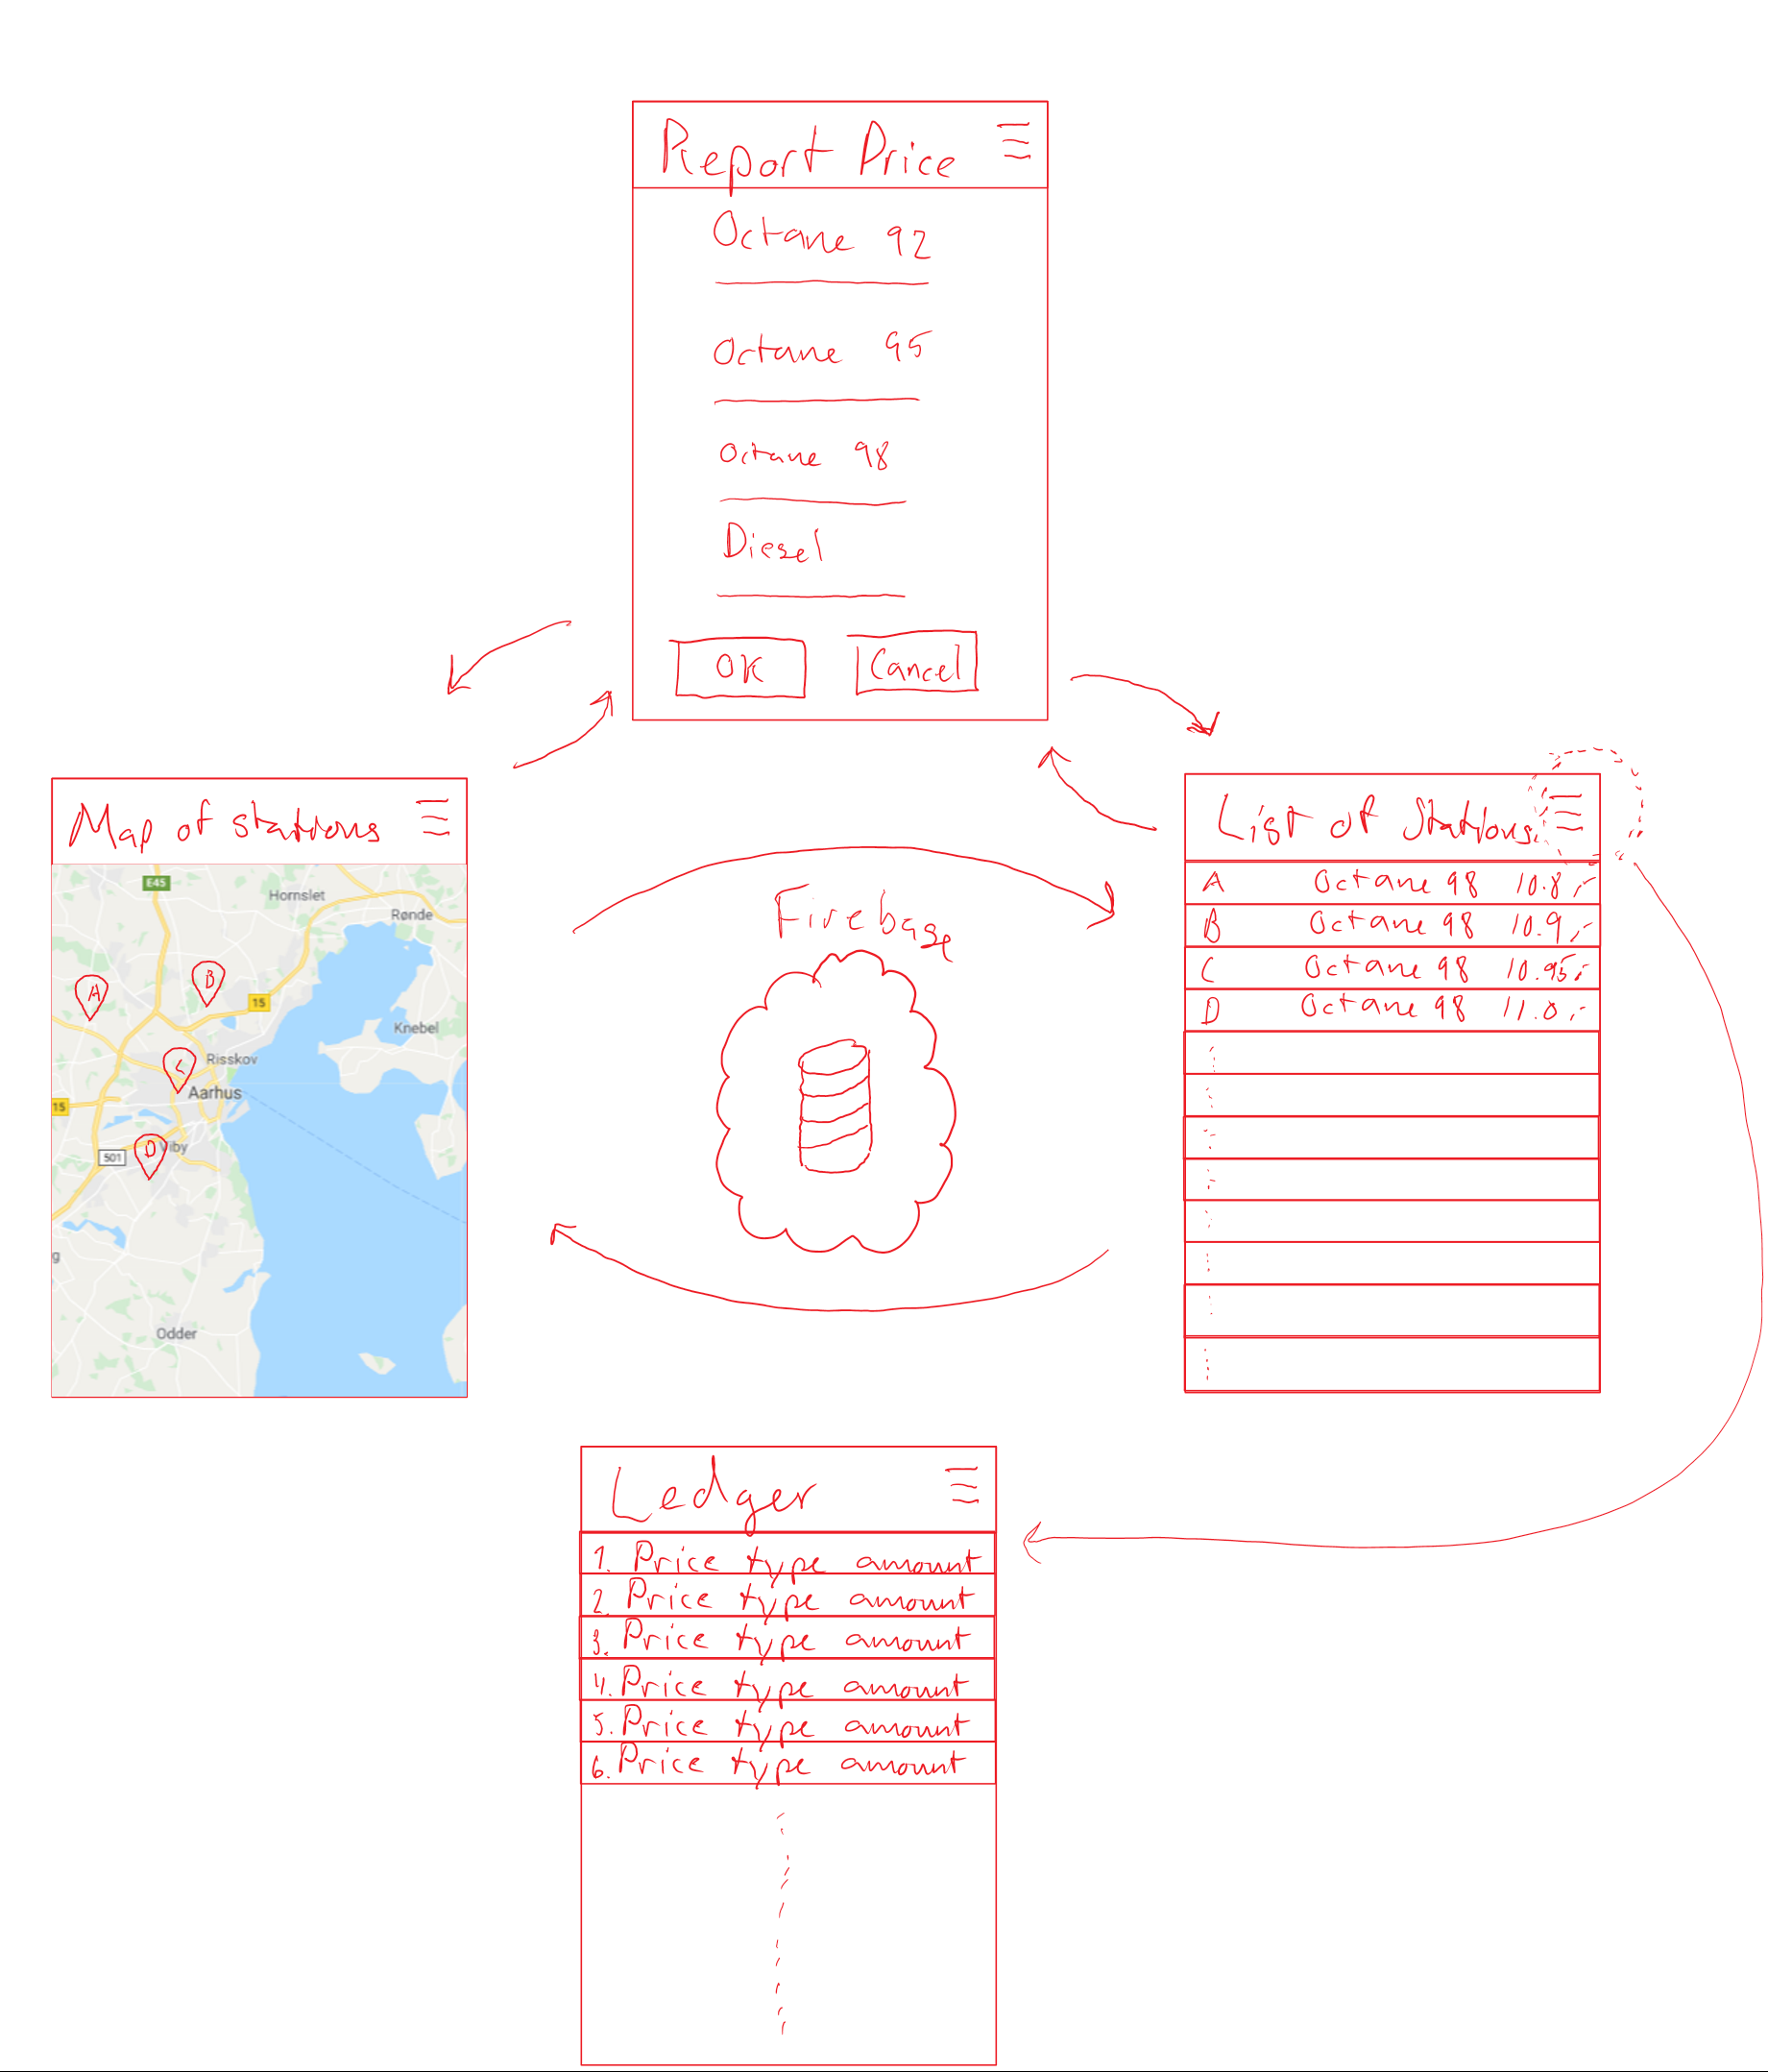
\includegraphics[width=0.95\textwidth]{P.png}
	\caption{Overview for the main portrait flow.}
	\label{fig:p}
\end{figure}

\begin{figure}[h]
	\centering
	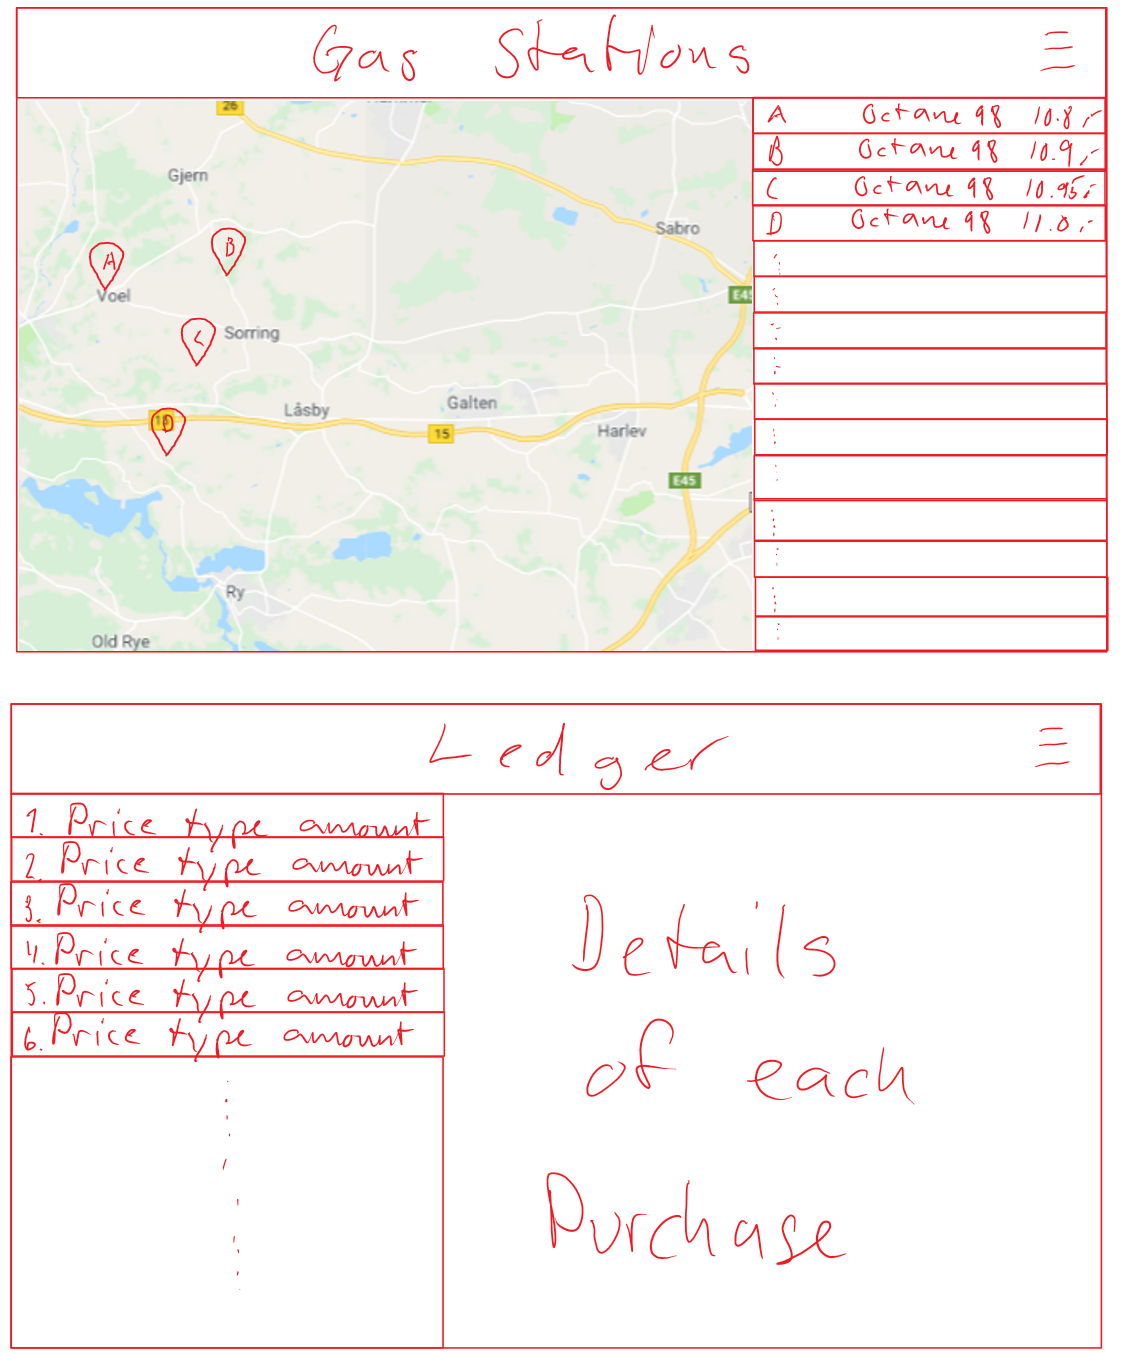
\includegraphics[width=\textwidth]{L.png}
	\caption{Overview for the main tablet/landscape flow.}
	\label{fig:l}
\end{figure}

\begin{figure}[h]
	\centering
	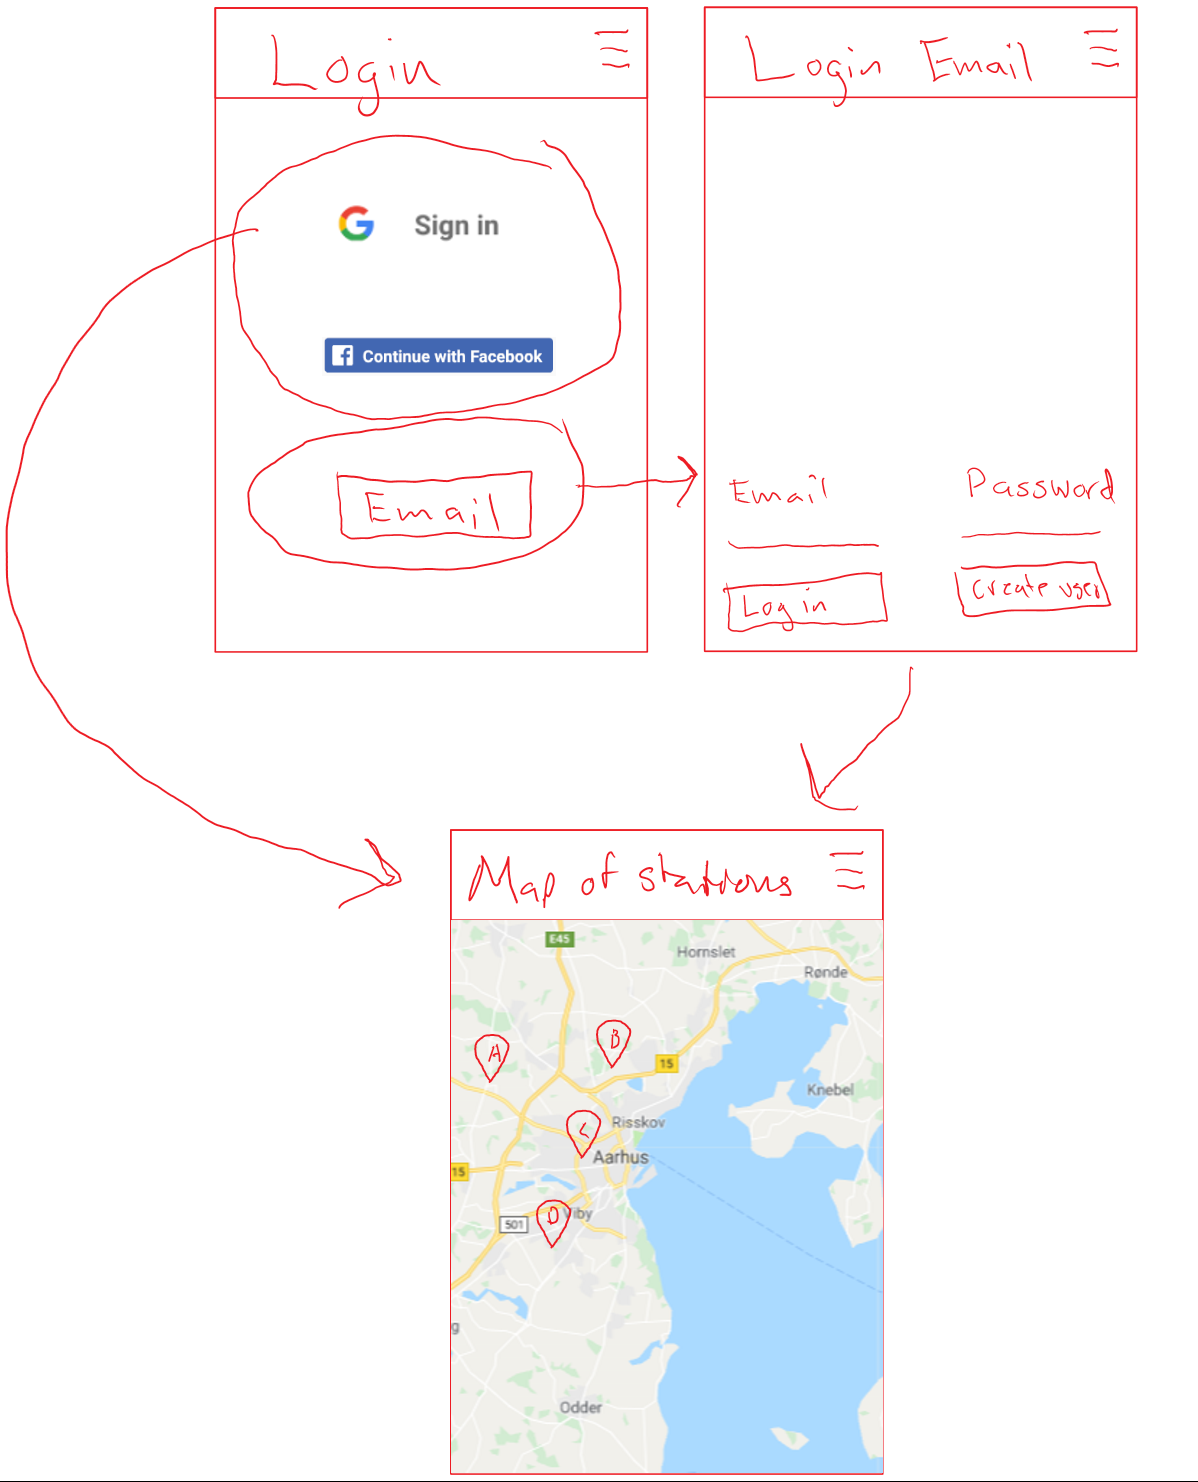
\includegraphics[width=\textwidth]{Login.png}
	\caption{Overview for the login flow. The design is similar for landscape and portrait, and only shown in one variation here.}
	\label{fig:login}
\end{figure}
